\chapter{Theory and Motivation}
\label{ch:2}

This chapter lays the theoretical groundwork on which the remainder of the thesis is built and gives insight to why the rare decay $D^0 \to \mu^+ \mu^-$ is a valuable probe for the new physics. The chapter begins with a short survey of Quantum Field Theory (QFT), outlining how the adoption of special relativity into qunatum mechanics gives rise to a QFT that is characterized by a Lagrangian and a resulting correlation function that can be calculated perturbatively. This framework then describes the computational tools for calculating these correlation function, such as path integrals, Feynman diagrams, the LSZ formulation, which allows the calculation of scattering amplitudes from correlation functions. 

Then, this chapter describes the Standard Model (SM), beginning with its local gauge symmetry structure and then building the fundamental particles and interactions from the resulting Lagrangian. Special attention is paid to the electroweak portion of the Lagrangian, giving an outline of the mechanism by which the Higgs field gives mass to the $W^\pm$ and $Z$ bosons, important mediators in the $D^0 \to \mu^+ \mu^-$ decay. 

Lastly, this chapter applies the theoretical groundwork established in its first two sections as a motivation for the $D^0 \to \mu^+ \mu^-$ search. Namely, flavor-changing neutral currents are defined and calculated to be not allowed at tree level in the SM. Loop contributions to the $D^0 \to \mu^+ \mu^-$ decay are cited to bring the branching fraction of the decay rate to $\simeq 10^{-13}$. The chapter ends by giving motivation as to why this makes the $D^0 \to \mu^+ \mu^-$ probe to new physics and giving a brief survey of the new physics that this probe could illuminate. 

\section{The Theory of Our Universe}

Since it's formulation in the early 1970's, the Standard Model of Particle Physics (SM) has become one of the most successful physics theories ever conceived. Not only does it describe 3 out of the 4 fundamental forces in our unniverse, but in the past 50 years it has explained virtually all small length scale experimental results and has made some of the most precise predictions in all of physics. For example, it predicted the discovery of the Higgs Boson that occurred in 2012 \cite{ref:cms2012observation}\cite{ref:atlas2012observation} and it predicted the anomalous magnetic dipole moment as $a = 0.00115965218059(13)$ \cite{ref:fan_2023}, which results into a prediction of the fine structure constant that has a precision of better than one part in a billion.

However we know that the SM cannot be the complete theory of our universe due to a few, major short comings. Perhaps the largest of these is the lack of gravity in it's description of physics, meaning it cannot describe any long distance cosmological observations. Other problems also persist at small length scales, such as the observation of neutrino oscillations \cite{ref:duan2010collective} which cannot occur using the massless neutrinos that the SM predicts. 

Therefore, physics analysis are often in search of Beyond the Standard Model (BSM) physics at small length scales to build a theory of particle physics that could solve many of the problems with the SM. Importantly, the SM is a quantum field theory, 

\section{Quantum Field Theory \cite{ref:harlow2024}}

Heuristically speaking, Quantum Field Theory (QFT) is a mathematical framework developed to unify the theories of classical special relativity and non-relavistic quantum mechanics. In the late 1920s, non-relativistic quantum mechanics had developed to a mature theory, modeling many of the phenomena that the physics of the 19th century simply couldn't explain. However, when put into context with Einstein's theory of special relativity, there were two central problems: 
\begin{enumerate}
    \item Velocities and momentums are strictly non relativistic 
    \item Interactions are instantaneous. 
\end{enumerate}
Fixing these two issues forces the fundamental building block of any QFT to be fields, not particles, that obey causality. Specifically, physics in a QFT is modeled as interactions between dynamical fields over spacetime coordinates.

In order to force compliance with special relativity and classical mechanics, the fields in any QFT must have 3 global symmetries:
\begin{enumerate}
    \item Translational symmetry along both spatial and temporal coordinates
    \item Rotational symmetry along two spatial coordinates
    \item Rotational symmetry along a spatial coordinate and the temporal coordinate
\end{enumerate}
The last symmetry gives rise to Lorentz transformation, which describe the invariance of inertial reference frames, one of the central properties of special relativity. These three global symmetries are often grouped together as Global Poincare Symmetry, which lays the framework for virtually all of QFT.

To construct a QFT, the Lagrangian is first written down as the most general Lagrangian possible that satisfies Global Poincare Symmetry as well as any local symmetries that should be preserved. Importantly, the Lagrangian must be renormalizable, meaning that divergences can be absorbed into the parameters of your model to give real, physical interpretations of the results.

\subsection{Correlation Functions}

Unfortunately, these Lagrangians can rarely be solved directly under the principle of least action. Instead, physicists study vacuum expectation values of time-ordered products of field operators, known as correlation functions. Using a path integral approach, one can write down the time ordered $n$-point correlation function of $\phi$ as
\begin{equation}
\braket{T \phi(x_{1}) \dots  \phi({x_{n}}))} = \frac{\int \mathcal{D}\phi \phi(x_{1}) \dots  \phi({x_{n}}) e^{iS_{\epsilon}}}{\int \mathcal{D}\phi e^{iS_{\epsilon}}}
\end{equation}
where $S_\epsilon$ is the action retrieved by integrating the Lagrangian over all of spacetime while analytically continuing time $t \to t - i\epsilon$ in order to force the exponential to converge. 
\begin{equation}
S_{\epsilon} = \int^{\infty(1-i\epsilon)}_{\infty(1-i\epsilon)} dt \int d^{d-1} x \mathcal{L}
\end{equation}
The path integral is evaluated by using perturbation theory to Taylor-expand the integral with respect to any coupling terms, resulting in integrals of the form 
\begin{equation}
\frac{\int d^{d-1}x x_{i_{1}}\dots x_{i_{n}} e^{-\frac{1}{2}x^TAx}}{\int d^{d-1}x  e^{-\frac{1}{2}x^TAx}}
\end{equation}
where $A$ is a symmetric matrix determined by the action $S_\epsilon$. This can be solved using derivatives in the complex vector, $B$, or the moments of the following gaussian integral:
\begin{equation}
\int d^{d-1} x e^{\frac{1}{2}x^TAx + B^Tx} = \frac{1}{\sqrt{ \det\left( \frac{A}{2\pi}\right) } } e^{\frac{1}{2}B^T A^{-1} B}
\end{equation}
The process of evaluating these integrals can be long and tedious. In the late 1940s, Richard Feynman introduced the Feynman Diagram as a graphical method for writing down these integrals along with Feynman Rules describing how to graphically evaluate correlation functions without needing to explicitly compute the path integral. While Feynman diagrams are often seen as "collision diagrams", it is important to remember their one-to-one relationship with path integrals of correlation functions. Once the Feynman Rules have been derived from the path integral of a specific QFT, they can be applied to get correlation functions. An example of a feynman diagram can be seen in figure \ref{fig:example_feynman_diagram}.

\begin{figure}[ht!]
    \centering
    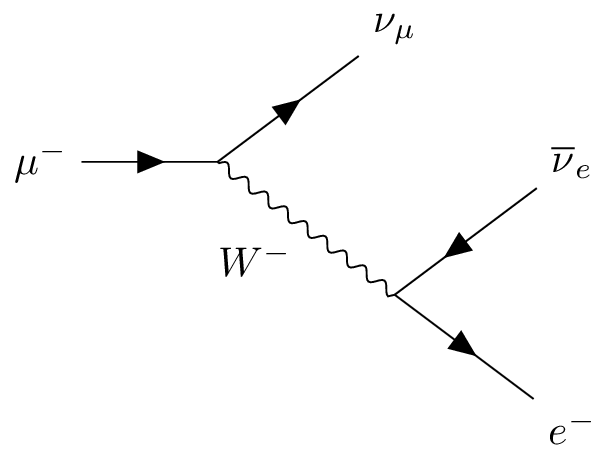
\includegraphics[width=0.4\textwidth]{figures/chapter2/example_feynman_diagram.png}
    \caption{An example feynman diagram describing the $\mu^- \to \nu_\mu \bar{\nu}_e e^-$ decay.}
    \label{fig:example_feynman_diagram}
\end{figure}

%**potentially should add section about propagators**

%**potentially should add a section about renormalization**

\subsection{Scattering}

While correlation functions are the foundational building block of theoretical QFT calculations, it is not immediately obvious with what to do with their result. Physicists think of particles instead of fields (such as in the SM) and are often interested in how they scatter off of one another. These scattering properties allow physicists to compute 
- Cross sections: roughly the rate at which a certain particle is produced.
- Branching fractions: the probability of a specific decay occurring, like is the subject of this thesis. 
which are the two most frequently measured quantities in colliders. So far, correlation functions have only given vacuum expectation values of field operators. 

Formalizing particles in a theory built on fields results in considering particles as eigenstates of the Hamiltonian whose wave packets are non-interacting at either early or late times, called "in" and "out" states respectively. A QFT can thus be equipped with a scattering description only if the Hamiltonian has a complete set of "in" and "out" states. Luckily, the SM is one such QFT.

The scattering properties between these "in" and "out" states can be extracted from the $S$-matrix, or the amplitude to find the world in an "out" state $\beta$, given that it started in an "in" state $\alpha$:
\begin{equation}
S_{\beta \alpha} = \braket{\beta|\alpha}   
\end{equation}
The method of constructing this $S$-matrix from correlation function is done using the LSZ Reduction Formula, which states that the existence of particles in a QFT leads to poles in the Fourier transform of its two-point functions (correlation functions between only two operators, also known as propagators). Therefore, computing the $S$-matrix amounts to computing correlation functions using Feynman Diagrams, taking the Fourier transform, taking all the external momentum to on-shell, and then computing the residue of the pole in the propagator. 

This thesis concerns itself with the branching fraction of the $D^0 \to \mu^+ \mu^-$ interaction. To compute the branching fraction from the scattering amplitude, it is first convenient to remove delta functions and constants always present in the scattering amplitude by defining the $M$-matrix as the matrix that satisfies
\begin{equation}
S_{\beta \alpha} = \delta(\beta -\alpha) + i \times(2\pi)^d \delta^d(p_{\beta}-p_{\alpha}) \mathcal{M}_{\beta \alpha}
\end{equation}
where $p_{\alpha}, p_{\beta}$ are the 4-momentum of the states. 

From this, one can calculate that the differential decay rate into a final state $\beta$ is given by
\begin{equation}
d \Gamma(\alpha \to \beta) = (2\pi)^d \delta^d(p_{\beta}-p_{\alpha}) |\mathcal{M}_{\beta \alpha}|^2 d \beta
\end{equation}
Specifically, to get a full decay width, one must integrate over all final states and their momentum that one cares about to get $\Gamma(\alpha \to \beta) = \int (2\pi)^d \delta^d(p_{\beta}-p_{\alpha}) |\mathcal{M}_{\beta \alpha}|^2 d \beta$. 

This concludes the outline of how to arrive at a branching fraction for a general QFT. The next section covers the specifics of the Standard Model as a QFT and the last section outlines the computation of the $D^0 \to \mu^+ \mu^-$ decay. 

\section{The Standard Model}

Recall that a QFT is constructed by identifying a list of local symmetries and then writing down the most general, renormalizable Lagrangian that satisfies the symmetries. The local symmetries of the SM are given by
\begin{equation}
SU(3) \times SU(2) \times U(1)
\end{equation}
Like many QFTs, there are two classifications of fields in the SM: bosons and fermions. While bosons are symmetric under exchange, fermions are antisymmetric under exchange. Consequently, the spin-statistic theorem states that fermions must have half integer spin while bosons have whole integer spin. Additionally, the spin-statistics theorem dictates that no two fermions may occupy the same state, making it very natural to think of them as matter. The total spin of two interacting half integer spin fermions must be whole integer, making it natural to think of bosons as mediators of interactions between fermions. 

The three local symmetries of the standard model are in fact gauge symmetries. They represent redundancy in description of our model, similar to the classical electromagnetism gauge. Due to some formalism we haven't developed and will leave out of this analysis, the generators of these gauge groups induce gauge bosons. Specifically, the 8 generators of $SU(3)$ give rise to the eight gluons that describe Quantum Chromodynamics (QCD) and the other four generators of $SU(2) \times U(1)$ give rise to electroweak (EW) interactions. Due to this, it makes sense to break up the LaGrangian into QCD and EW terms, which we know can be written independently, due to the independence of their generators. Namely, we have that
\begin{equation}
\mathcal{L}_{SM} = \mathcal{L}_{EW} + \mathcal{L}_{QCD}
\end{equation}
In the following sections, we will analyze each of these LaGrangians independently, showing how they give rise to the various particles in the SM and their interactions. As a preview, the particles of the standard model and their quantum numbers are summarized in figure \ref{fig:particles_of_the_SM}. 

\begin{figure}[ht!]
    \centering
    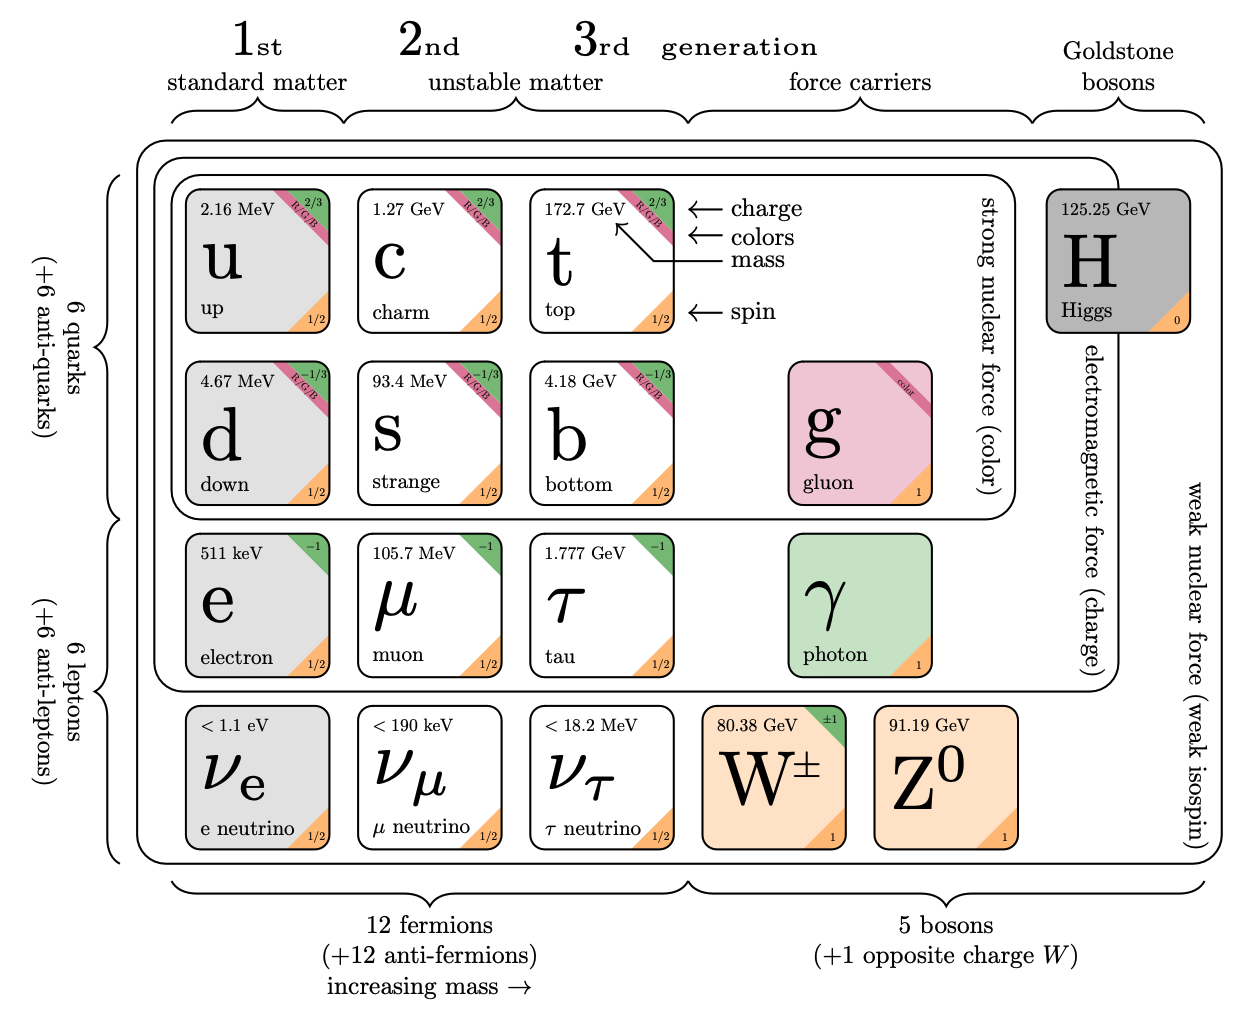
\includegraphics[width=0.8\textwidth]{figures/chapter2/particles_of_the_SM.png}
    \caption{The particles of the standard model}
    \label{fig:particles_of_the_SM}
\end{figure}

\subsection{Quantum Chromodynamics}

The eight generators of $SU(3)$ are given by the Glenn-Mann matrices and yield the 8 bosons of QCD, known as gluons. The three-dimensional basis of these matrices give rise to 3 colors, labeled $r$, $g$, and $b$ as well as their opposites $\bar{r}, \bar{g}, \bar{b}$, which are the fundamental charges of QCD. The Glenn-Mann matrices govern that each of the gluons can carry a color and an anti-color charge. The corresponding fermions in this theory are named quarks and simply carry one color charge or one anti-color charge for anti-quarks. There are 6 different flavors of quarks, summarized in table \ref{tab:quark_masses}. 

\begin{table}[htbp]
    \centering
    \begin{tabular}{@{}lccc@{}}
      \toprule
      Quark & Symbol & Charge $Q/e$ & Mass (MeV/$c^{2}$) \\ 
      \midrule
      Up     & $u$ & $+2/3$ & $2.16^{+0.49}_{-0.26}$ \\
      Down   & $d$ & $-1/3$ & $4.67^{+0.48}_{-0.17}$ \\
      Charm  & $c$ & $+2/3$ & $1270 \pm 20$ \\
      Strange& $s$ & $-1/3$ & $93^{+11}_{-5}$ \\
      Top    & $t$ & $+2/3$ & $172\,760 \pm 300$ \\
      Bottom & $b$ & $-1/3$ & $4180^{+30}_{-20}$ \\
      \bottomrule
    \end{tabular}
    \caption{Electric charge and mass of the six quark flavours.
             Masses are quoted in the schemes recommended by the
             Particle Data Group\,\cite{ref:pdg2024}.}
    \label{tab:quark_masses}
  \end{table}


By constructing a QFT that is invariant under $SU(3)$, one arrives at the LaGrangian
\begin{equation}
    \mathcal{L}_{{QCD}} = \bar{q}^a\cancel{D}_{ab}q^b - m_{ab}\bar{q}^aq^b - \frac{1}{4}G^a_{\mu\nu}G_a^{\mu\nu}
\end{equation}
where $q_i$ is the quark field, with $i$ being the flavor index which is implicitly summed over all the quark flavors. $\cancel{D}$ is a contraction between the gauge covariant derivative and the gamma matrices $\gamma^\mu$ which connect the spinor representation of the fields to the vector representation of the Lorentz group. Stated explicitly, we have
\begin{equation}
    \cancel{D} = \gamma^\mu (D_\mu)_{ab} = \gamma^\mu\left( \partial_\mu \delta_{ab}  - ig_s(G_\mu)_{ab}\right)
\end{equation}
where $G_\mu$ is the gauge field and represented by the Glann-Mann matrices and $g_s$ is the strong coupling constant found in renormalization. $G_{\mu\nu}$ is the associated field strength tensor, given by
\begin{equation}
G_{\mu\nu} = \partial_\mu G_\nu - \partial_\nu G_\mu - ig_s[G_\mu, G_\nu]
\end{equation}
Lastly, $m_{ij}$ resembles the mass matrix of the various quark flavors and is only non-zero when $i=j$.

In general, perturbative calculations in QCD can be quite complex and difficult. Therefore, in practice, QCD is often place on a lattice, imposing a hard momentum cut-off and performing perturbations on the lattice. 

\subsection{Electroweak Interactions}

The electromagnetic and weak nuclear forces are unified under EW interactions at energies above $\approx 250 \text{ GeV}$ or temperatures above $\approx10^{15}$\textdegree $K$, mediated by the $SU(2) \times U(1)$ symmetry. The generators of the $SU(2)$ group yield three gauge bosons of weak isospin, given by $A^i_{\mu}$, and the generators of the $U(1)$ group yeild three gauge bosons of of weak hypercharge, given by $B_{\mu}$. Importantly, $SU(2)$ is the chiral part of the electroweak symmetry, meaning it only affects left-handed fermions. Therefore, much of the discussion on electroweak interactions will differentiate between left handed and right handed particles.

Due to spontaneous symmetry breaking, the four vector bosons are mixed using the Weinberg angle, $\theta_W$, to produce the 4 physical gauge bosons: $\gamma$, $Z^0$, $W^\pm$. Note that the photon, $\gamma$ is sometimes written as the electromagnetic field $A_{\mu}$ and is not to be confused the weak isospin gauge bosons, $A_\mu^i$. Additionally, the $Z^0_{\mu}$ is often just written as $Z_{\mu}$, dropping the charge label. Specifically, the mixing under the Weinberg angle manifests as
\begin{equation}
    \begin{split}
    W^\pm_{\mu} &= \frac{1}{\sqrt{2}}(A^1_{\mu} \mp i A^2_{\mu}) \\
    \begin{pmatrix}
        A_{\mu} \\ Z^0_{\mu}
    \end{pmatrix} &= 
    \begin{pmatrix}
        \cos\theta_W & \sin\theta_W \\
        -\sin\theta_W & \cos\theta_W
    \end{pmatrix}
    \begin{pmatrix}
        B_{\mu} \\ A^3_{\mu}
    \end{pmatrix}
    \label{eq:Weinberg_mixing}
\end{split}
\end{equation}
    

The left handed fermions in this theory are given as doublets that transform under $SU(2) \times U(1)$ and can be categorized into leptons and quarks. Specifically the doublet notation is used to manifestly ensure transformation under $SU(2)$. This is similar to a two-state quantum spin system with $\ket{0} = \begin{pmatrix} 1 \\ 0 \end{pmatrix}$ and $\ket{1} = \begin{pmatrix} 0 \\ 1 \end{pmatrix}$ with spin operators that act as $SU(2)$ rotations on the spin vectors. The components of these doublets are the $U(1)$ abiding states, similar to those given by QED interactions.

Therefore, the left handed leptons are given by
\begin{equation}
L_{i} = \begin{pmatrix}
\nu_{iL} \\ l_{iL}
\end{pmatrix}
\end{equation}
where $\nu_{iL}$ are the three left handed neutrinos and the $l_{iL}$ particles are the three other left handed leptons. Notationally, we use $i$ to sum over all three flavors and $L$ to denote the left-handedness of the field. Left handed quarks are given by
\begin{equation}
Q_{i} = \begin{pmatrix}
u_{iL} \\ V_{ij} d_{jL}
\end{pmatrix}
\end{equation}
where $u_{iL}$ are the the three up quarks, $d_{iL}$ are the three down quarks, and $V_{ij}$ is the Cabibbo-Kobayashi-Maskawa (CKW) matrices that keep track of the Weinberg angle mixing coefficients.

The right handed fermions in this theory are not affected by the $SU(2)$ symmetry; they only transform trivially due to the chirality assigned to the $SU(2)$ symmetry. Therefore, right handed states are $SU(2)$ singlets that must only abide by $U(1)$ symmetry. We write these to be $u_{iR}$, $d_{iR}$, and $e_{iR}$. However, for notational ease, often the $R$ is dropped since all the left fields are in doublets. Therefore, we write the quark fields as $u_{i}$, $d_{i}$, and $e_{i}$.

\subsubsection{The Higgs field}

Now, there is one more subtly that must be addressed before introducing the LaGrangian for the electroweak interaction. Specifically, we know that in $d=4$, renormalizable QFTs can only contain non-invariant dimension-four operators, meaning that it cannot allow a term that would give mass to the bosons, such as $m^2 B_{\mu}^aB^{a\mu}$ for the weak isospin gauge bosons.  This is consistent with our formulation of QCD above due to the massless gluon, as well as consistent with our observation of the massless photon. However, the $W^\pm$ and $Z$ boson are observed to carry mass.

Therefore, we must introduce a scalar field that is allowed to break the $SU(2) \times U(1)$ symmetry and give rise to $Z$ and $W^\pm$ masses. This field is known as the Higgs field. While an in-depth discussion of the Higgs mechanism is out of the scope of this thesis, a short discussion should suffice to understand the EW LaGrangian.

In order to give mass to the $W^\pm$ and $Z$ bosons, the field we add must allow for the full LaGrangian to remain invariant while resulting in a ground state that is not. One good way to think of this is known as the mexican hat potential, given by $f(r, \theta) = (r^2 - v^2)$ shown in figure \ref{fig:mexican_hat_potential}. This potential is completely rotationally symmetric, but the ground state lies away from the origin at $r = v$, meaning the ground state itself is not spherically symmetric. Additionally it satisfies all other properties of a valid potential by being continuous, well defined, and bounded from below. Therefore, we introduce a doublet under $SU(2)$, given by
\begin{equation}
h = \begin{pmatrix}
h^+ \\ h^0
\end{pmatrix}
\end{equation}
and put it in the mexican hat potential. 

\begin{figure}[ht!]
    \centering
    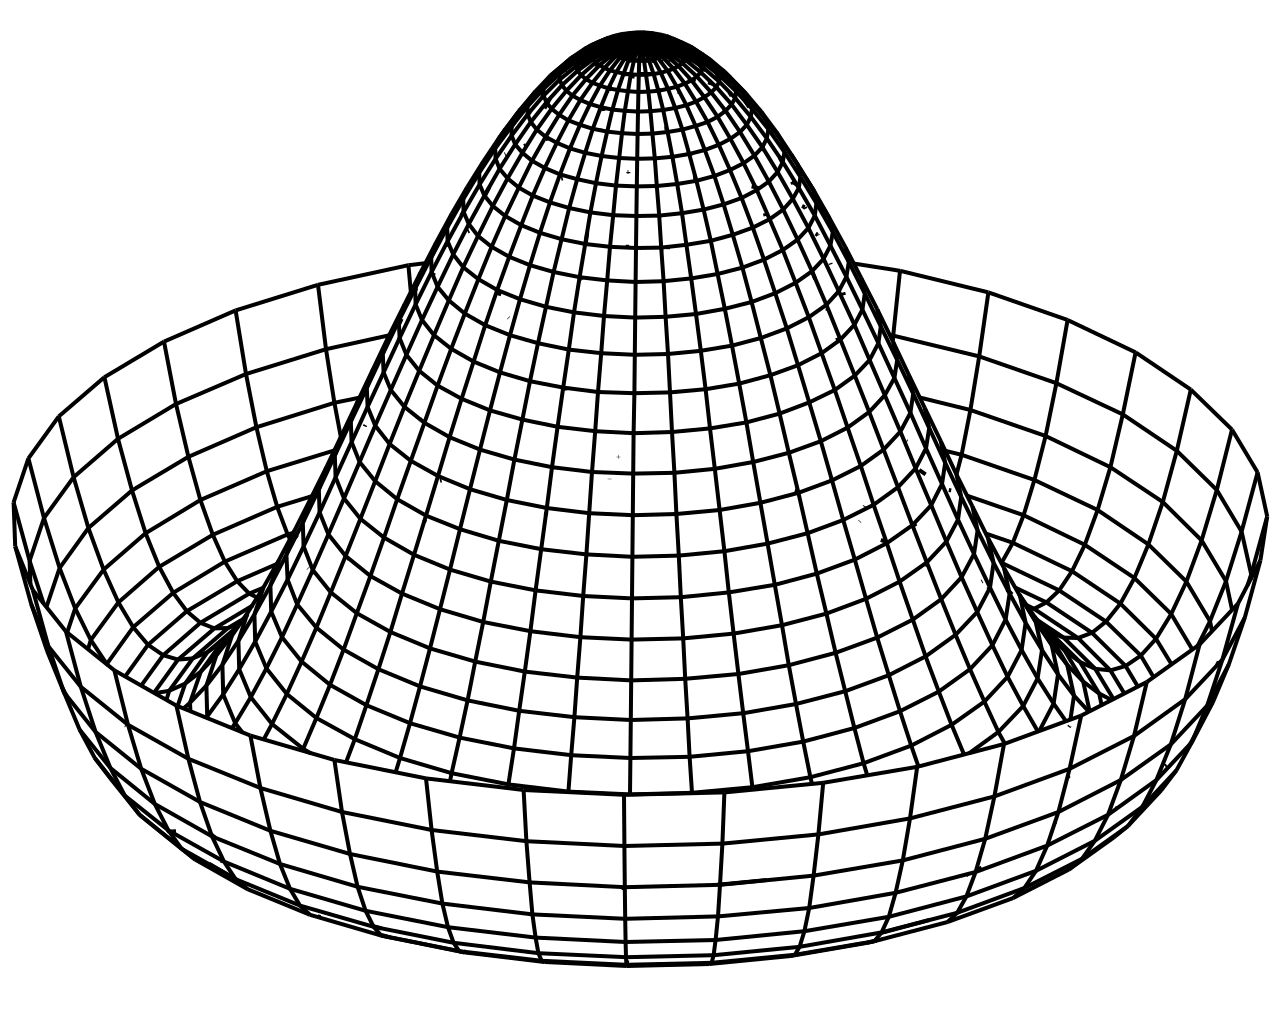
\includegraphics[width=0.4\textwidth]{figures/chapter2/mexican_hat_potential.png}
    \caption{The mexican hat potential, given by $f(r, \theta) = (r^2 - v^2)$, demonstrating ground state symmetry breaking in a symmetric potential}
    \label{fig:mexican_hat_potential}
\end{figure}

To see that indeed this gives the $W$ and $Z$ bosons mass, we write down the LaGrangian of this field in the presence of the $W^a_\mu$ and $B_\mu$ fields as
\begin{equation}
\mathcal{L}_{h} = (D_{\mu}h)(D^\mu h) - \lambda\left(|h|^2- \frac{v}{2}\right)^2
\label{eq:higg-field-lagrangian}
\end{equation}
where $D_\mu = (\partial_\mu - \frac{ig}{2}\tau^a A^a_\mu - \frac{ig'Y}{2}B_\mu)$. Here $\tau^a$ (also known as the Pauli matrices) and $YI$ are the generators of $SU(2)$ and $U(1)$. Their corresponding eigenvalues are labeled as $T_a$\footnote{$T_a$ is actually the eigenvalue of $\frac{\tau^a}{2}$} and $Y$; they are known as the weak isospin and weak hypercharge quantum numbers and a convenient basis is often $T^2 = T_1^2 + T_2^2 + T_3^2$, $T_3$, and $Y$. Separately, note that $\lambda\left(|h|^2- \frac{v}{2}\right)^2$ is exactly a rescaled mexican hat potential. Now, it is straight forward to see that this LaGrangian contains the terms
\begin{equation}
\frac{v^2}{8}\left[g^2\left((A^{1}_{\mu})^2 + (A^{2}_{\mu})^2\right) + (gA_{\mu}^3 - g' B_{\mu})\right]
\end{equation}
giving the intermediate weak isospin and weak hypercharge bosons mass. Using the Weinberg angle and letting $\tan(\theta_W) = g'/g$, the mass terms of the observed bosons become
\begin{equation}
M_{W^+} = M_{W^-} = \frac{gv}{2} \quad\quad M_{Z} = \frac{gv}{2\cos(\theta_{W})} \quad\quad M_{\gamma} = 0
\end{equation}

\subsubsection{Full Electroweak Theory}

Finally, by constructing a QFT involving these fields and one that is invariant under $SU(3)$, one arrives at the LaGrangian
\begin{equation}
\mathcal{L}_{EW} = \mathcal{L}_{g} + \mathcal{L}_{f} + \mathcal{L}_{h} + \mathcal{L}_{y}
\end{equation}
were $\mathcal{L}_g$ is the gauge term, similar to the QCD gauge term, given by
\begin{equation}
\mathcal{L}_g = -\frac{1}{4}A^i_{\mu\nu}A^{i\mu\nu} - \frac{1}{4} B_{\mu\nu} B^{\mu\nu}
\end{equation}
The electroweak field strength tensors $A^i_{\mu\nu}$ and $B_{\mu\nu}$ are defined similarly to how the gluon field tensor is defined for QCD.

$\mathcal{L_f}$ is the fermion kinetic term, given by
\begin{equation}
\mathcal{L}_{f} = \bar{L}_{i}\cancel{D}L_{i} + \bar{e}_{i}\cancel{D}e_{i} + \bar{Q}\cancel{D}Q + \bar{u} \cancel{D}u + \bar{d}\cancel{D}d
\label{eq:fermion_kinetic_term}
\end{equation}
where again $\cancel{D}$ is the covariant derivative in the above section, $D_\mu$ contracted with a gamma matrix, $\gamma^\mu$ and the fields are defined in the above section as left handed doublets and right handed singlets.

$\mathcal{L}_h$ has already been defined in the previous section and $\mathcal{L}_Y$ are the Yukawa interaction terms between the fermion fields and the higgs scalar field. This is given by
\begin{equation}
\mathcal{L}_{y} = - Y_{e} \bar{L}he + Y_{u}\bar{Q}h u + Y_{d} \bar{Q}h d
 + \text{h.c.}
\end{equation}
Here, for notational convience we have dropped the flavor indices. $Y_{e,u,d}$ are the three yukawa interaction term matrices. Similar to how the higg field gives the $W^\pm$ and $Z$ bosons mass, this is how the fermions gain mass in electroweak theory. 

\section{The $D^0 \to \mu^+ \mu^-$ decay.}

In principal, now that we have written down the SM Lagrangian, one could follow the standard QFT formalism described above to calculate perturbitively $\Gamma(D^0 \to \mu^+ \mu_-)$. In practice, this is incredibly complex and involves decades of perturbative QFT formalisms. Therefore, in this section we will first categorize this decay as a flavor changing neutral current --describing it's significance as such-- and heuristically summarize the calculation of $\mathcal{B}(D^0 \to \mu^+ \mu^-)$ done by G. Burdman, E. Golowich, J. L. Hewett, and S. Pakvasa (BGHP) \cite{ref:burdman_2002}.

\subsection{Flavor Changing Neutral Currents}

Flavor changing neutral currents (FCNCs) are interactions that change the flavor of a fermion without altering it's electric charge. 

The SM forbids flavor-changing neutral currents expicitly at tree level. Processes that are flavor-changing with neutral currents must first undergo a flavor change in a loop which combines to give a neutral current, the details of which are discussed later. To see explicitly why this is true, we start with the gluon-fermion interaction terms of the LaGrangian which we derived earlier. Namely we have that the interaction terms can be pulled out of equation \ref{eq:fermion_kinetic_term} to give us
\begin{equation}
\mathcal{L}_{gf} = \sum_{f=\{ Q, L, u, d, e\}} \bar{f}_{i} \gamma^\mu \left(\partial_\mu - \frac{ig}{2} \tau^a A^a_\mu - ig' \frac{Y}{2} B_\mu\right)f_{i}
\end{equation}
Now, we begin to rotate into the Weinberg frame, using $\tau^\pm = \frac{\tau^1 \pm i\tau^2}{\sqrt{2}}$ and $W^\pm$ defined as in equation \ref{eq:Weinberg_mixing}. This gives us
\begin{equation}
\mathcal{L}_{gf} = \sum_{f=\{ Q, L, u, d, e\}} \bar{f}_{i} \gamma^\mu \left(\partial_\mu - \frac{ig}{\sqrt{2}} (W^+_\mu\tau^+ + W_\mu^- \tau^-) -\frac{g}{2} A^3_\mu\tau^3 - \frac{g'}{2}B_\mu Y\right)f_{i}
\end{equation}
From this, we can easily isolate $\mathcal{L}_{gf}$ into neutral currents and charged currents, as $\tau^\pm$ is the charged operator.\footnote{This fact is not explicitly proven here, but can be shown by writing out $\tau^\pm$ in the doublet basis and then noticing that $\tau^+$ converts the lower component into the upper one while $\tau^-$ does the opposite. This causes the weak isospin eigenvalue to change while keeping hypercharge constant, resulting a change in electric charge, $Q = I_3 + Y/2$} Therefore, we have that the neutral current interactions are given by
\begin{equation}
\mathcal{L}_{NC} = \sum_{f=\{ Q, L, u, d, e\}} \bar{f}_{i} \gamma^\mu \left( -\frac{g}{2} A^3_\mu\tau^3 - \frac{g'}{2}B_\mu Y\right)f_{i}
\end{equation}
Now, we notice that the LaGrangian only has interactions between fermions with the same flavor index. Therefore, the only flavor mixing that can occur is between the doublets. Therefore, we can expand out to get the candidates for FCNC interactions as
\begin{equation}
\begin{split}
\mathcal{L}_{\text{FCNC Candidates}} = &-\frac{g}{2}\begin{pmatrix}
\bar{u}_{iL} & \bar{d_{iL}}
\end{pmatrix} \gamma^\mu A_{\mu}^3 \begin{pmatrix}
1 & 0 \\ 0 & -1
\end{pmatrix} \begin{pmatrix}
u_{iL} \\ d_{iL}
\end{pmatrix} \\
&-\frac{g}{2}\begin{pmatrix}
\bar{\nu}_{iL} & \bar{l_{iL}}
\end{pmatrix} \gamma^\mu A_{\mu}^3 \begin{pmatrix}
1 & 0 \\ 0 & -1
\end{pmatrix} \begin{pmatrix}
\nu_{iL} \\ l_{iL}
\end{pmatrix} \\
&-\frac{g'}{2}\begin{pmatrix}
\bar{u}_{iL} & \bar{d_{iL}}
\end{pmatrix} \gamma^\mu B_{\mu} \begin{pmatrix}
1 & 0 \\ 0 & 1
\end{pmatrix} \begin{pmatrix}
u_{iL} \\ d_{iL}
\end{pmatrix} \\
&-\frac{g'}{2}\begin{pmatrix}
\bar{\nu}_{iL} & \bar{l_{iL}}
\end{pmatrix} \gamma^\mu B_{\mu} \begin{pmatrix}
1 & 0 \\ 0 & 1
\end{pmatrix} \begin{pmatrix}
\nu_{iL} \\ l_{iL}
\end{pmatrix}
\label{eq:large-eq-for-FCNC-candidates}
\end{split}
\end{equation}
Now, we can consolidate this significantly by introducing $e = g\sin(\theta_W) = g'\cos(\theta_W)$\footnote{The second equality can be verified by using $\tan(\theta_W) = \frac{g'}{g}$}, $A^3_\mu = \cos(\theta_W)Z_\mu + \sin(\theta_W)A_\mu$, and $B_\mu = -\sin(\theta_W)Z_\mu + \cos(\theta_W) A_\mu$. The second two equations can be derived from equation \ref{eq:Weinberg_mixing}. Additionally, we can use the weak isospin and weak hypercharge eigenvalues $I_3$ and $Y$, defined below equation \ref{eq:higg-field-lagrangian}.  It is also useful to define the electric charge eigenvalue, $Q = I_3 + Y/2$. Using this, we can simply equation \ref{eq:large-eq-for-FCNC-candidates} greatly as
\begin{equation}
\begin{split}
\mathcal{L}_{\text{FCNC Candidates}} &= -\sum_{f = u_{L},d_{L},l_{L}, \nu_{L}} \left[\frac{e}{\sin(\theta_{W})\cos(\theta_{W})} \bar{f}_{i}\gamma^\mu Z_{\mu}\left(T_{3}^{(f)} -Q^{(f)}\sin^2(\theta_{W})\right)\bar{f}_{i}\right]\\
&- \sum_{f = u_{L},d_{L},l_{L}, \nu_{L}} \left[ e \bar{f}_{i}\gamma^\mu A_{\mu}Q^{(f)}f_{i}\right]
\end{split}
\end{equation}
where the values of $T_3^{(f)}$, $Y^{(f)}$ and $Q^{(f)}$ can be found in table \ref{tab:ew_charges}. 


\begin{table}[htbp]
    \centering
    \begin{tabular}{|lccc|lccc|}
      \hline
      \multicolumn{4}{|c|}{\textbf{Left‑handed fermions}} &
      \multicolumn{4}{c|}{\textbf{Right‑handed fermions}} \\
      \hline
      Field & $T_3$ & $Y$ & $Q/e$ &
      Field & $T_3$ & $Y$ & $Q/e$ \\
      \hline
      Up quark $u_L$        & $+1/2$ & $+1/3$ & $+2/3$ &
      Up quark $u_R$        & $0$    & $+4/3$ & $+2/3$ \\
      Down quark $d_L$      & $-1/2$ & $+1/3$ & $-1/3$ &
      Down quark $d_R$      & $0$    & $-2/3$ & $-1/3$ \\
      Neutrino $\nu_L$      & $+1/2$ & $-1$   & $0$    &
      Charged lepton $l_R$  & $0$    & $-2$   & $-1$   \\
      Charged lepton $l_L$  & $-1/2$ & $-1$   & $-1$   &
                            &        &        &        \\
      \hline
    \end{tabular}
    \caption{Weak isospin $(T_3)$, weak hypercharge $(Y)$, and electric
             charge $(Q)$ for the chiral fermions of one Standard‑Model
             generation\,\cite{ref:pdg2024}.}
    \label{tab:ew_charges}
  \end{table}
  
  

More importantly, we notice that there are indeed no FCNC terms left. More specifically, there are no terms that allow for interactions between fermions of two different flavors. Therefore, we have that $\mathcal{L}_{FCNC} = 0$ under the SM, preventing FCNC at tree level. 

\subsection{The $D^0 \to \mu^+ \mu^-$ decay as a FCNC}

Hadrons, such as the $D^0$ are collections of quarks in bound states. One defining property of QCD is that virtually all hadrons are in gluon-bound color-neutral states. These states therefore contain either a quark and an antiquark (known as baryons) or a quark and an antiquark (known as mesons). $D$ mesons are known a *charm mesons* and are any light meson that contains a charm quark. The $D^0$ is one such meson, being the only neutrally charge $D$ meson, composed of a *charm* and an *anti-up* quark. Note that there is also an anti-$D^0$ meson, being composed of an *anti-charm* and an *up* quark. 

Now, since the $D^0$ meson is composed of a quark pair and the final state $\mu^+ \mu^-$ contains no quarks, therefore indicating that there must be a flavor change. However, importantly the $D^0$ is a neutral particle, as is the $\mu^+, \mu^-$ final state. Therefore, for there to be a tree-level contribution, there must be a tree-level FCNC, which is not allowed by the standard model. Therefore, the $D^0 \to \mu^+ \mu^-$  decay must involve many vertices and is thus heavily suppressed by the standard model.

G. Burdman, E. Golowich, J. L. Hewett, and S. Pakvasa (BGHP) have carried out the most complete SM analysis of the $D^0 \to \mu^+ \mu^-$ decay that includes all short and long-distance effects. 

To begin with the short distance (SD) effects, the quark level transition arises from electroweak penguin and box diagrams, an example of which is found in Feynman diagram in figure ??. After integrating over all possible diagrams, BGHP find that 
\begin{equation}
\mathcal{B}(D^0 \to \mu^+ \mu^-)_{SD} \simeq 10^{-18}
\end{equation}

TODO: add feynman diagram

Next, BGHP identify two distinct long distance (LD) mechanisms, single-particle unitary contributions and two-photon contributions. The single particle unitary contributions are dominated by weak-mixing with ground-state presudoscalars, such as $\pi^0, \eta, \eta'$, followed by these pseudoscalars decaying into a dimuon final state, $P^0 \to \mu^+ \mu^-$. The branching fraction of this calculation is given by
\begin{equation}
\mathcal{B}(D^0 \to \mu^+ \mu^-)_{\pi^0, \eta, \eta'} \simeq 2.5 \times 10^{-18}
\end{equation}
In principal, there could be mixing with heavier $0^\pm$ resonances such as $\pi(1800)$, however the decays of $\pi(1800) \to \mu^+\mu^-$ occur with a branching fraction likely around $10^{-12}$, leading to
\begin{equation}
\mathcal{B}(D^0 \to \mu^+ \mu^-)_{\pi(1800)} \simeq  5.0 \times 10^{-17}
\end{equation}
The two-photon contributions come from the dispersive two photon decay $D^0 \to \gamma \gamma \to \mu^+ \mu^-$. BGHP show that 
\begin{equation}
\mathcal{B}(D^0 \to \mu^+ \mu^-)_{\gamma\gamma} \simeq 2.7 \times 10^{-5} \mathcal{B}(D^0 \to \gamma\gamma)
\end{equation}
where their own calculations show that, by considering short distance contributions, long distance vector meson dominant contributions, long distance single particle unitary contributions, and long distance two-particle unitary contributions, $\mathcal{B}(D^0 \to \gamma\gamma) \simeq 10^{-8}$. Therefore, 
\begin{equation}
\mathcal{B}(D^0 \to \mu^+ \mu^-)_{\gamma\gamma} \simeq 10^{-13}
\end{equation}
When summing each of these contributions, one finds that $\mathcal{B}(D^0 \to \mu^+ \mu^-)_{\gamma\gamma} \simeq 10^{-13}$ is by far the largest, therefore BGHP conclude that
\begin{equation}
\mathcal{B}(D^0 \to \mu^+ \mu^-)_{\text{total}} \simeq 10^{-13}
\end{equation}
It is also worth noting that BGHP show that various new physics models significantly increase this branching fraction. However, their work on this is far out of the scope of this thesis and outlines many different new physics models, including many commonly accepted candidates for Beyond the Standard Model (BSM) physics such as Flavor Non-Universal Z' Bosons and Super Symmetry (SUSY). One such model is Flavor Non-Universal Z' Bosons, which introduce neutral Z' bosons with flavor off diagonal couplings 

Due to the complexity and number of these models, we simply refer to their work to give meaningful calculations in support of new physics should a branching fraction significantly larger than $10^{-13}$ be detected. It should be clear from these calculations that putting better limits on $\mathcal{B}(D^0 \to \mu^+ \mu^-)$ acts as a meaningful probe into many new physics models, serving as the primary motivation of this work. 